%\appendix{Related Publications}
\begin{appendices}
\chapter{Texture Description with Local Binary Patterns}
\label{AppendixA}

The Local Binary Pattern (LBP) operator is defined as a gray-scale invariant texture measure, derived from a general definition of texture in a local neighborhood. Originally, the LBP texture descriptor \cite{ojala1996comparative}, was computed in a pixel level basis using a $3 \times 3$ kernel, thresholding the surroundings of each pixel with the central pixel value and considering the result as a binary value. The decimal form of the LBP code is expressed as:

\begin{equation}
LBP(x_{c},y_{c})=\displaystyle\sum\limits_{n=0}^{N-1} \emph{f}(i_{n}-i_{c})2^n,
\label{eq:LBP}
\end{equation}
\noindent where $i_{c}$ corresponds to the gray intensity of the center pixel ($x_{c}, y_{c}$), $N$ is the number of sampling points, $i_{n}$ is the gray intensity of the n-th surrounding pixel, and $f(x)$ is defined as follows:

\begin{equation}
f(x)  =
\left\lbrace \begin{array}{ccc}
0 & \mbox{if} & x<0 \\
1 & \mbox{if} & x\geq0 
\end{array}. \right.
\label{eq:fx}
\end{equation}

\cite{ojala2002multiresolution} extended this operator to support surrounding points and radius of a pixel neighbourhood with different shapes and sizes, enabling handling textures at different scales. Fig. \ref{fig_lbpOperator} illustrates the operator calculation and the points distribution in a circular neighbourhood with radius 2, where the pixel values are bilinearly interpolated whenever the sampling point is not in the center of a pixel.

\begin{figure}
\begin{center}
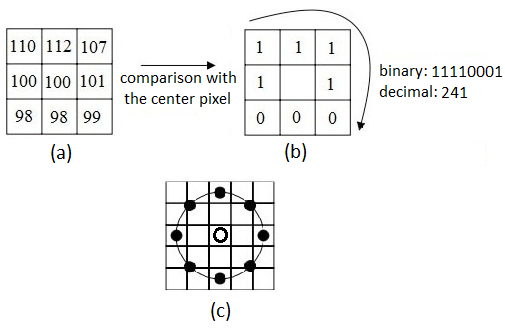
\includegraphics [width=7.5cm] {images/lbp_operator}
\caption[LBP operator]{LBP operator. (a) and (b) The basic LBP operator, where the neighbourhood of each pixel is thresholded and a binary number is obtained. (c) A circular neighbourhood example (with 8 neighbour points and radius 2). The pixel values are bilinearly interpolated whenever the sampling point is not in the center of a pixel.} \label{fig_lbpOperator}
\end{center}
\end{figure}

Another important extension proposed by \cite{ojala2002multiresolution} was the uniform patterns concept ($u2$). A LBP operator is considered uniform if it contains at most two bitwise transitions 0-1 or 1-0 when viewed as a circular bits chain. According to \cite{ojala2002multiresolution}, nearly 90 percent of LBP operators observed in face images are uniform. In spacial terms, uniform patterns represent some patterns of a texture: spot, flat, area, edge and corner. With an 8-bit representation, there are 58 patterns with at most two bitwise transitions. Fig. \ref{fig_uniformPattern}, extracted from \cite{chan2007multi}, describes all possible uniform patterns with 8 neighbours.

\begin{figure}
\begin{center}
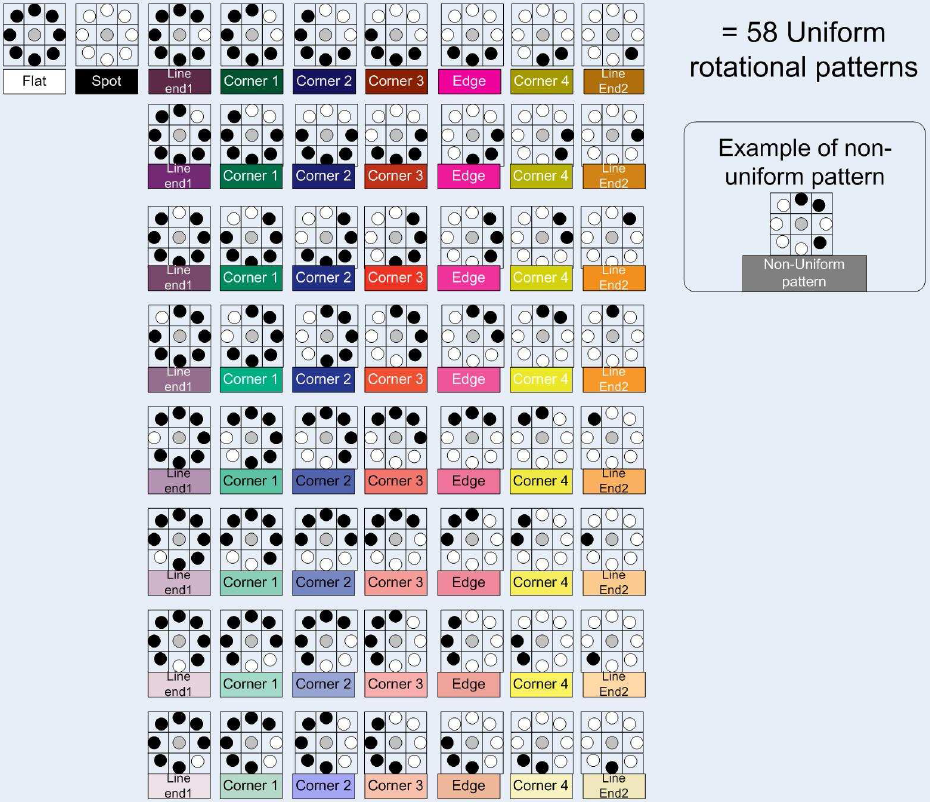
\includegraphics [width=12cm] {images/fig_uniformPattern} 
\end{center}
   \caption[All uniform patterns for LBP with 8 neighbours]{All uniform patterns for LBP with 8 neighbours \cite{chan2007multi}.}   
\label{fig_uniformPattern}
\end{figure}

\cite{ahonen2004face} and \cite{ahonen2006face} adopt the following notation for the LBP operator: $LBP_{P,R}^{u2}$, where the subscript represents the neighbourhood configuration with $P$ sampling points on a circle of radius $R$, and the superscript $u2$ stands for using only uniform patterns and labelling all non-uniform patterns with a single label.


\chapter{Related Publications}
\label{AppendixB}

During this masters dissertation, were published the following papers:

\begin{enumerate}[I.]
	\item PEREIRA, T. F.; DE MARTINO, J. M. Dete\c{c}\~ao de ataques de spoofing em sistemas de autentica\c{c}\~ao de faces que utilizam webcams. Quinto Encontro dos Alunos e Docentes do Departamento de Engenharia de Computa\c{c}\~ao e Automac\~ao Industrial - EADCA 2012, 26-27 de abril de 2012, Faculdade de Engenharia El\'etrica e de Computa\c{c}\~ao - Unicamp, Campinas, SP, Brasil. 2012. p. 77-80.

	\item Freitas Pereira, Tiago ; Anjos, Andr\'e ; Martino, Jos\'e Mario ; Marcel, S\'ebastien . LBP-TOP Based Countermeasure against Face Spoofing Attacks. Lecture Notes in Computer Science. 1ed.: Springer Berlin Heidelberg, 2013, v. , p. 121-132.;

	\item PEREIRA, T. F. ; ANJOS, A. R. ; MARTINO, J. M. ; MARCEL, S. . Can face anti-spoofing countermeasures work in a real world scenario?. In: 6th IAPR International Conference on Biometrics (ICB2013), 2013, Madrid, Spain. 6th IAPR International Conference on Biometrics (ICB2013), 2013.

	\item CHINGOVSKA, I. YANG, J. LEI, Z. YI, D. LI, S. Z. KAHM, O. GLASER, C. DAMER, N. KUIJPER, A. NOUAK, A. KOMULAINEN, J. PEREIRA, T. F. GUPTA, S. KHANDELWAL, S. BANSA, S. RAI, A. KRISHNA, T. GOYAL, D. WARIS, M. ZHANG, H. AHMAD, I. KIRANYAZ, S. GABBOUJ, M. TRONCI, R. PILI, M. , et al. ; The 2nd Competition on Counter Measures to 2D Face Spoofing Attacks. In: 6th IAPR International Conference on Biometrics (ICB2013),, 2013, Madrid, Spain. 6th IAPR International Conference on Biometrics (ICB2013),, 2013.

	\item FREITAS PEREIRA, T.; KOMULAINEN, J; ANJOS, A. R. ; MARTINO, J. M.;  HADID, A.;  PIETIK{\"A}INEN, M.; MARCEL, S. . Face liveness detection using dynamic texture,/ In:. EURASIP Journal on Image Processing and Video Processing \footnote{Under editorial decision making};  




 
\end{enumerate}

\end{appendices}